\subsection{Universities: Visions of
Utopia}\label{universities-visions-of-utopia}

If the university campus lived up to its potential it could be a true
paradise: essentially a giant garden filled with buildings for studying
and creating knowledge. Amazing! They are usually situated on some of
the best land to be found anywhere, have great access to everything
needed in life, and have dense urban style housing in a pastoral
environment which allows for a simple, car free life.

\subsection{Brief History of the
University}\label{brief-history-of-the-university}

Where did the universities come from?

Looking up sources at UAA library.

The universities of Europe, 1100-1914 : a history is at LA627.R82 1984

\subsection{Undergraduate Education: Broken
Promises}\label{undergraduate-education-broken-promises}

\subsection{Grad School: The Ponzi
Scheme}\label{grad-school-the-ponzi-scheme}

\subsection{Hollowing Out of the
Academy}\label{hollowing-out-of-the-academy}

\subsection{Intellectual Property}\label{intellectual-property}

\subsection{Potential Paradises}\label{potential-paradises}

\subsection{University Occupations, Phase
2}\label{university-occupations-phase-2}

\subsection{Case Study: Yale
University}\label{case-study-yale-university}

\begin{itemize}
\tightlist
\item
  How much land owned?
\item
  How much is arable?
\item
  How much is already zoned for ag?
\item
  What water resrouces are there?
\item
  number of staff, students, alumni, faculty
\item
  How many people could Yale support?
\item
  Holdings outside New Haven
\item
  Yale Singapore
\item
  Repurposing the Endowment, total divestment from capitalism
\item
  political and legal process of re-writing the charter of the school,
  changing governance
\end{itemize}

yale history:
https://www.worldcat.org/title/yale-university/oclc/40331263\&referer=brief\_results

yale land holdings:

\url{http://sustainability.yale.edu/planning-progress/areas-focus/landscape}

\subsection{Case Study: University of
Paris(Sorbonne)}\label{case-study-university-of-parissorbonne}

https://en.wikipedia.org/wiki/University\_of\_Paris

https://en.wikipedia.org/wiki/University\_of\_Paris\_strike\_of\_1229

\begin{figure}[htbp]
\centering
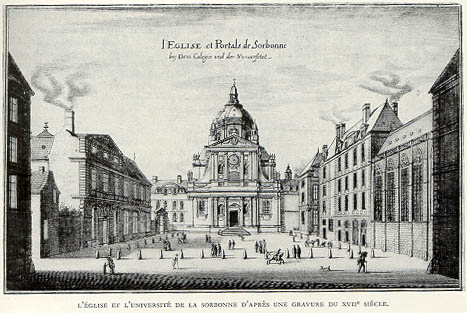
\includegraphics{images/Sorbonne_17thc.jpg}
\caption{image}
\end{figure}

\subsubsection{this chapter should have a section with a detailed
example}\label{this-chapter-should-have-a-section-with-a-detailed-example}

maps, tables, really dig in and figure out the strategy and tactics that
could be used, maybe have multiple examples, small liberal arts, huge
public school, elite private school, community college in a big city

\subsubsection{The Universities are a
Disaster}\label{the-universities-are-a-disaster}

\begin{itemize}
\item
  Academia as pyramid scam
\item
  Academia as tool of the military industrial State
\item
  Academia as a marketing tool for the banking cartel
\item
  Academia: where ideas go to die
\item
  Academia: it was here before capitalism and it will be here after
\item
  Has traditionally been a part of various religions and patriarchal
  systems connected with them
\end{itemize}

IP is key to how bad it is, academia after the re-occupation of the
campus all property will be banned from campus.

\subsubsection{But they're really useful to
us}\label{but-theyre-really-useful-to-us}

Back to basics: knowledge, teaching, philosophy, technology, culture,
books, land, food and energy

Universities must be Occupied and declared independent

This should be across disciplines and outside of the capitalist class
system, bringing in workers, locals, students, teachers, researchers and
everyone else involved. Seize the legal control of the corporation that
is the University, and you will have a power that States must respect.

Taking universities over can be a huge international beach head that
goes around all national borders.

Important reference:

Universities, Inc.

call number: 338.43378 WASHBURN

DPL description:

``Our federal and state tax dollars are going to fund higher education.
If corporations kick in a little more, should they be able to dictate
the research or own the discoveries?During the past two decades,
commercial forces have quietly transformed virtually every aspect of
academic life. Corporate funding of universities is growing and the
money comes with strings attached. In return for this funding,
universities and professors are acting more and more like for-profit
patent factories: university funds are shifting from the humanities and
the less profitable science departments into research labs, and the
skill of teaching is valued less and less. Slowly but surely,
universities are abandoning their traditional role as disinterested
sources of education, alternative perspectives, and wisdom.This growing
influence of corporations over universities affects more than just
today's college students (and their parents); it compromises the future
of all those whose careers depend on a university education, and all
those who will be employed, governed, or taught by the products of
American universities.''
